% !TEX root = ../OT4ML.tex

%%%%%%%%%%%%%%%%%%%%%%%%%%%%%%%%%%%%%%%%%%%%%%%%%%%%%%%%%%%%%%%%%%%%%%%%%%%
%%%%%%%%%%%%%%%%%%%%%%%%%%%%%%%%%%%%%%%%%%%%%%%%%%%%%%%%%%%%%%%%%%%%%%%%%%%
%%%%%%%%%%%%%%%%%%%%%%%%%%%%%%%%%%%%%%%%%%%%%%%%%%%%%%%%%%%%%%%%%%%%%%%%%%%
\section{Advanced Topics on Entropic Regularization}
\label{sec-sinkhorn-advanced}

This section collects the refinements that make entropic OT practical and statistically meaningful. It develops the dual smooth problem, revisits convergence, introduces the debiased Sinkhorn divergence and explains why regularization improves sample complexity. These topics connect algorithm design~\cite{cuturi2018semidual,2017-carlier-SIMA} with modern statistical uses of regularized OT~\cite{genevay2018sample,feydy2018interpolating}.

%%%%%%%%%%%%%%%%%%%%%%%%%%%%%%%%%%%%%%%%%%%%%%%%%%%%%%%%%%%%%%%%%%%%%%%%%%%
\subsection{Dual of Sinkhorn}

The dual point of view replaces couplings by potentials and soft $c$-transforms. It is the right formulation for stabilized implementations and differentiation.

%%%
\paragraph{Discrete dual.}

The following proposition details the dual problem associated to~\eqref{eq-regularized-discr}.

\begin{prop}[Dual of entropic OT]
One has
\eql{\label{eq-dual-formulation}
	\MKD_\C^\epsilon(\a,\b) = \umax{\fD \in \RR^n,\gD \in \RR^m}
		 \dotp{\fD}{\a} + \dotp{\gD}{\b}
		% - \epsilon\sum_{i,j} e^{ \frac{\fD_i+\gD_j-\C_{i,j}}{\epsilon} }.
%		- \epsilon \dotp{e^{\fD/\epsilon} }{ \K e^{\gD/\epsilon}}.
	- \epsilon \sum_{i,j} \exp\pa{
		\frac{\fD_i+\gD_j-\C_{i,j}}{\epsilon}
	} \a_i \b_j + \epsilon.
}
%
The optimal $(\fD,\gD)$ are linked to scalings $(\uD,\vD)$ appearing in~\eqref{eq-scaling-form} through
\eql{\label{eq-entropy-pd}
		\uD_i=\a_i e^{\fD_i/\epsilon}
		\qandq
		\vD_j=\b_j e^{\gD_j/\epsilon}.
}
\end{prop}

\begin{proof}
We introduce Lagrange multipliers and consider
\eq{
	\umin{\P \geq 0} \umax{\fD,\gD} \dotp{\C}{\P} + \epsilon \KLD(\P|\a \otimes \b) + \dotp{\a-\P\ones}{\fD} + \dotp{\b-\P^\top\ones}{\gD}.
}
	Finite-dimensional convex duality allows us to exchange the minimum over $\P$ with the maximum over $(\fD,\gD)$, giving
	\eq{
		 \umax{\fD,\gD}
		 \dotp{\fD}{\a} + \dotp{\gD}{\b}
		 +
		 \epsilon \umin{\P \geq 0}
		 \pa{
			\KLD(\P|\a \otimes \b)
			-
			\dotp{\frac{\fD\oplus\gD-\C}{\epsilon}}{\P}
		 }
			=
			\dotp{\fD}{\a} + \dotp{\gD}{\b} - \epsilon \KLD^*\pa{ \frac{\fD\oplus\gD-\C}{\epsilon}|\a \otimes \b }.
	}
	One concludes by using~\eqref{eq-legendre} for $\phi(r)=r \log(r)-r+1$
	\eq{
		\KLD^*(H|\a \otimes \b) = \sum_{i,j} \phi^*(H_{i,j}) \a_i \b_j.
	}
	Indeed, the scalar maximization
	\[
		\phi^*(s)=\sup_{r\geq0}\{rs-r\log r+r-1\}
	\]
	has first-order condition $s-\log r=0$, hence $r=e^s$ and $\phi^*(s)=e^s-1$.
	\end{proof}

%%%
\paragraph{Discrete soft $c$-transforms.}

Since the dual problem~\eqref{eq-dual-formulation} is smooth and concave, one can perform alternating block maximization. For a fixed $\gD$, maximizing with respect to $\fD$ leads to the following equation after zeroing the derivative with respect to $\fD$:
\eq{
	\a_i - e^{\frac{\fD_i}{\epsilon}} \a_i \sum_j \exp\pa{
		\frac{\gD_j-\C_{i,j}}{\epsilon}
	} \b_j = 0
}
which leads to the explicit solution
\eq{
	\fD_i = -\epsilon \log \sum_j \exp\pa{ \frac{\gD_j-\C_{i,j}}{\epsilon} } \b_j.
}
We conveniently introduce the soft-min operator of some vector $h \in \RR^m$
\eq{
	{\min}_{\b}^\epsilon(h) \eqdef -\epsilon \log \sum_j e^{-h_j/\epsilon} \b_j
}
which is a smooth approximation of the minimum operator, and the optimal $\fD$ for a fixed $\gD$ is computed by a soft version of the $c$-transform
\eql{\label{eq-soft-c-1}
	\fD_i = {\min}_{\b}^\epsilon( \C_{i,\cdot} - \gD ).
}
In a similar way, the optimal $\gD$ for a fixed $\fD$ is
\eql{\label{eq-soft-c-2}
	\gD_j = {\min}_{\a}^\epsilon( \C_{\cdot,j} - \fD ).
}
Exponentiating these iterations recovers exactly the Sinkhorn algorithm. These iterations, however, become unstable for small $\epsilon$. To apply the algorithm in this regime, one needs to stabilize it using the celebrated log-sum-exp trick. This follows from noticing that, similarly to the minimum operator, one has
\eq{
	{\min}_{\b}^\epsilon(h-\text{cst})={\min}_{\b}^\epsilon(h)-\text{cst}
}
and to replace the computation of ${\min}_{\b}^\epsilon(h)$ by its stabilized version (equal when using infinite precision computation) ${\min}_{\b}^\epsilon(h-\min(h)) + \min(h)$.


\paragraph{Other regularizers.}

The exponential form of Sinkhorn scalings is specific to KL regularization. Other convex penalties on the density of $\P$ with respect to $\a\otimes\b$ lead to the same marginal constraints but to different pointwise transfer laws.
For an entropy $h:\RR_+\to\RR\cup\{+\infty\}$ and $\lambda>0$, consider
\[
	\umin{\P\in\CouplingsD(\a,\b)}
	\dotp{\C}{\P}
	+\lambda\sum_{i,j}\a_i\b_j\,
	h\!\left(\frac{\P_{i,j}}{\a_i\b_j}\right),
\]
assuming for simplicity that $\a_i,\b_j>0$.

\begin{prop}[Pointwise laws for entropy-regularized plans]
	Let $\P$ be an optimal plan for the preceding problem and let $(\fD,\gD)$ be dual multipliers for the two marginal constraints. With
	\[
		r_{i,j}\eqdef \frac{\P_{i,j}}{\a_i\b_j},
		\qquad
		s_{i,j}\eqdef \frac{\fD_i+\gD_j-\C_{i,j}}{\lambda},
	\]
	one has $s_{i,j}\in\partial h(r_{i,j})$. In the smooth interior this reads $r_{i,j}=(h')^{-1}(s_{i,j})$. In particular,
	\[
	\begin{array}{lll}
		h(r)=r\log r-r+1 &\Rightarrow& r_{i,j}=e^{s_{i,j}},\\[.25em]
		h(r)=r-\log r-1 &\Rightarrow& r_{i,j}=(1-s_{i,j})^{-1}\quad (s_{i,j}<1),\\[.25em]
		h(r)=\frac12(r-1)^2 &\Rightarrow& r_{i,j}=(1+s_{i,j})_+.
	\end{array}
	\]
\end{prop}

\begin{proof}
	Introduce Lagrange multipliers in the form
	\[
		\dotp{\C}{\P}
		+\lambda\sum_{i,j}\a_i\b_j h(r_{i,j})
		+\dotp{\a-\P\ones}{\fD}
		+\dotp{\b-\P^\top\ones}{\gD}.
	\]
	The stationarity condition with respect to $\P_{i,j}$ gives
	\[
		0\in \C_{i,j}-\fD_i-\gD_j+\lambda\partial h(r_{i,j}),
	\]
	which is the announced inclusion. The three displayed formulas follow by inverting $h'$ for KL and Burg. For the quadratic penalty, the unconstrained solution is $1+s_{i,j}$ and the constraint $r_{i,j}\geq0$ projects it to its positive part.
\end{proof}

\begin{figure}[ht]
\centering
\setlength{\tabcolsep}{2pt}
\begin{tabular}{@{}ccc@{}}
\small KL entropy & \small Burg barrier & \small quadratic density penalty \\[-.15em]

\includegraphics[width=.31\linewidth]{figures/sinkhorn-entropic-versus-quadratic-regularization/kl-plan.pdf} &

\includegraphics[width=.31\linewidth]{figures/sinkhorn-entropic-versus-quadratic-regularization/burg-plan.pdf} &

\includegraphics[width=.31\linewidth]{figures/sinkhorn-entropic-versus-quadratic-regularization/quadratic-plan.pdf}
\end{tabular}
\caption{Effect of the regularizing entropy on the coupling. The red and blue side curves are fixed one-dimensional Gaussian-mixture marginals. The central matrix displays the square root of the coupling density on a common color scale. KL regularization gives the usual diffuse positive plan, the Burg barrier keeps a positive but differently tailed support, and the quadratic density penalty can set entries exactly to zero through its positive-part law.}
\label{fig:sinkhorn-entropic-versus-quadratic-regularization}
\end{figure}


\begin{rem}[Gaussian rates]\label{rem-gaussian-rates}
	Because the Sinkhorn iterates remain quadratic, Gaussian Sinkhorn reduces to a finite-dimensional nonlinear iteration on means and covariance parameters. In the centered one-dimensional case with both marginals equal to $\Gaussian(0,1)$ and kernel $K_\epsilon(x,y)=e^{-(x-y)^2/\epsilon}$, write one scaling as $v_k(y)=\exp(-q_k y^2+\mathrm{cst})$. The next row scaling is again Gaussian, with quadratic coefficient
	\[
		F(q_k)
		=
		\frac1\epsilon
		-
		\frac{1}{\epsilon^2(q_k+\frac12+\frac1\epsilon)}.
	\]
	One full Sinkhorn cycle is therefore $q_{k+1}=F(F(q_k))$. If $q_\star=F(q_\star)$ and $B_\star=q_\star+\frac12+\frac1\epsilon$, then
	\[
		B_\star^2-\left(\frac12+\frac2\epsilon\right)B_\star+\frac1{\epsilon^2}=0,
		\qquad
		F'(q_\star)=\frac{1}{\epsilon^2 B_\star^2}.
	\]
	The local linear rate for one full cycle is thus $(F'(q_\star))^2$. This explicit scalar formula shows the same qualitative behavior as the general Gaussian analysis of Chizat, Delalande and Va\v{s}kevi\v{c}ius~\cite{chizat2024sharper}: the rate improves when $\epsilon$ is large and deteriorates as $\epsilon$ becomes small, where the entropic coupling approaches a deterministic Brenier map.
\end{rem}


%%%%%%%%%%%%%%%%%%%%%%%%%%%%%%%%%%%%%%%%%%%%%%%%%%%%%%%%%%%%%%%%%%%%%%%%%%%
\subsection{Convergence Analysis}
\label{sec-convergence-dual}

This subsection revisits Sinkhorn convergence through three complementary lenses. Hilbert's metric gives a clean contraction, Fortet's order argument gives qualitative fixed-point convergence, and robust Bregman estimates give a non-asymptotic $O(1/k)$ dual-gap bound. The first two viewpoints explain asymptotic convergence mechanisms, while the last one is often the most useful for explicit complexity estimates.

\paragraph{Hilbert-metric linear convergence.}

The Hilbert metric convergence result is equivalent to convergence on the dual potentials $(f,g)$ according to the variation norms. For bounded cost $c$ (e.g. on compact spaces),
\eq{
	\norm{f_k-f^\star}_V = O(\la^k)
	\qandq
		\norm{g_k-g^\star}_V = O(\la^k)
}
\eq{
	\norm{ \log \frac{\d\pi_k}{\d\pi^\star} }_\infty
	=
	\norm{ (f_k-f^\star) \oplus (g_k-g^\star) }_\infty
	\leq
	\norm{f_k-f^\star}_V + \norm{g_k-g^\star}_V
}
where the contraction ratio is the Birkhoff factor of the Gibbs kernel $\K_\epsilon=e^{-c/\epsilon}$. Namely, with $\eta=\eta(\K_\epsilon)$ as in Theorem~\ref{thm-birkhoff} and $R\eqdef\sup c-\inf c$,
\[
	\la=\frac{\sqrt{\eta}-1}{\sqrt{\eta}+1}
	\leq
	\tanh(R/(2\epsilon))<1 .
\]
One also has the following bounds
\eq{
	\norm{f_k-f^\star}_V \leq \frac{ \norm{\log\frac{\d \pi_{k,1}}{\d\al}}_\infty }{1-\la}
}
which can be used to provide a posterior estimate of the rate of convergence and serve as a stopping criterion.


%%%
\paragraph{Order-monotone convergence.}

There is another, older way to understand convergence, going back to Fortet's proof of the Schr\"odinger system~\cite{fortet1940schrodinger,essid2019fortet,leonard2019fortet}. It does not primarily estimate a contraction factor. Instead, it uses the order structure of the soft transforms.

\begin{prop}[Monotone fixed-point route to Sinkhorn convergence]\label{prop-fortet-monotone}
	Let $c$ be bounded and continuous on compact spaces, and define the double Sinkhorn map, normalized by subtracting its $\alpha$-mean,
	\[
		\mathcal A(f) \eqdef
		(f^{c,\epsilon})^{\bar c,\epsilon}
		-\int (f^{c,\epsilon})^{\bar c,\epsilon}\d\alpha.
	\]
	The map $\mathcal A$ is order preserving modulo additive constants. If an initialization is chosen so that $f_0\leq \mathcal A(f_0)$ after normalization, then the iterates $f_{k+1}=\mathcal A(f_k)$ increase pointwise up to constants, remain uniformly bounded in oscillation, and converge to a fixed point. A convenient practical choice is $f_0=0$, followed if necessary by subtracting a sufficiently large constant so that the subsolution inequality holds. This fixed point is the entropic potential, hence the associated Sinkhorn scalings converge.
\end{prop}

\begin{proof}
	The soft $c$-transform is order reversing: if $g\leq g'$, then
	\[
		-\epsilon\log\int e^{(g-c)/\epsilon}\d\beta
		\geq
		-\epsilon\log\int e^{(g'-c)/\epsilon}\d\beta.
	\]
	The composition of two order-reversing transforms is therefore order preserving. The transform also commutes with additive constants in the projective sense, which is why one fixes a normalization. Starting from a subsolution gives $f_0\leq f_1$, and order preservation gives $f_k\leq f_{k+1}$ for all $k$. Soft-transform oscillation bounds, controlled by $\sup c-\inf c$, prevent escape to infinity after normalization. Monotone pointwise convergence, compactness of equicontinuous soft transforms, and continuity of $\mathcal A$ then give a fixed point. Uniqueness of entropic potentials up to constants, Proposition~\ref{prop-entropic-unique} and the dual uniqueness statement above identify this fixed point with the Sinkhorn solution.
\end{proof}

This proof is qualitative rather than quantitative, but it is conceptually useful: Sinkhorn is not only alternating projection or projective contraction; it is also a monotone fixed-point iteration on potentials once constants are quotiented out.


%%%
\paragraph{Robust sublinear Bregman rate.}

	Sinkhorn is cyclic coordinate ascent on the smooth dual problem and, equivalently, alternating KL projection on the two marginal constraint sets. We denote the continuous entropic dual objective by
	\eql{\label{eq-dual-sinkh-cont}
		\mathcal D_\epsilon(f,g)
		\eqdef
		\int f\d\alpha+\int g\d\beta
		-\epsilon\int\left(e^{(f\oplus g-c)/\epsilon}-1\right)\d\alpha\otimes\d\beta .
	}
	The following statement records the rate that is most useful for complexity estimates: before entering a possible linear regime, the dual objective gap decreases at order $1/k$. We state it for balanced entropic OT, which is the specialization needed here; related robust Bregman-projection rates are developed in~\cite{peyre2026robust,altschuler2017near,pmlr-v80-dvurechensky18a}, and statistical consequences of entropic smoothing are analyzed in~\cite{genevay2018sample,bigot2017central}.

\begin{prop}[Pinsker inequality]\label{prop-pinsker}
	If $p,q\in\simplex_n$, then
	\[
		\norm{p-q}_1^2 \leq 2\KL(p|q).
	\]
\end{prop}
\begin{proof}
	It is enough to prove the scalar inequality
	\[
		u\log u-u+1 \geq \frac{(u-1)^2}{2(u+1)}
		\qquad u\geq0.
	\]
	Indeed, after bringing the right-hand side to the left, the resulting function $h$ satisfies $h(1)=h'(1)=0$ and, for $u>0$,
	\[
		h''(u)=\frac1u-\frac{4}{(u+1)^3}
		=
		\frac{(u+1)^3-4u}{u(u+1)^3}\geq0,
	\]
	so $h$ is convex and minimized at $u=1$.
	Multiplying by $q_i$ and summing with $u=p_i/q_i$ gives, first when all $q_i>0$ and then by approximation in general,
	\[
		\KL(p|q)
		\geq
		\frac12\sum_i\frac{(p_i-q_i)^2}{p_i+q_i}.
	\]
	Cauchy--Schwarz yields
	\[
		\norm{p-q}_1^2
		=
		\left(\sum_i\frac{|p_i-q_i|}{\sqrt{p_i+q_i}}\sqrt{p_i+q_i}\right)^2
		\leq
		\left(\sum_i\frac{(p_i-q_i)^2}{p_i+q_i}\right)
		\left(\sum_i(p_i+q_i)\right),
	\]
	and $\sum_i(p_i+q_i)=2$.
\end{proof}

\begin{prop}[A compact $O(1/k)$ dual rate]\label{prop-sinkhorn-dual-rate}
	Assume that $\Xx$ and $\Yy$ are compact, that $c$ is bounded, and write $R=\sup c-\inf c$. Let $(f_k,g_k)$ be Sinkhorn dual iterates normalized by $\int f_k\d\alpha=0$, and let
	\[
		\Delta_k
		\eqdef
		\mathcal D_\epsilon(f^\star,g^\star)-\mathcal D_\epsilon(f_k,g_k)
	\]
	be the dual suboptimality gap for the entropic dual objective~\eqref{eq-dual-sinkh-cont}. Then there exists a numerical constant $C$ such that
	\[
		\Delta_k \leq \frac{C R^2}{\epsilon(k+1)}.
	\]
\end{prop}

\begin{proof}
	The proof uses three elementary ingredients. First, the soft $c$-transform bounds the oscillation of every normalized iterate and every normalized optimum:
	\[
		\norm{f_k}_V+\norm{g_k}_V+\norm{f^\star}_V+\norm{g^\star}_V \leq C R.
	\]
	Here $\norm{h}_V\eqdef\sup h-\inf h$ is the variation seminorm, the same projective norm used in Hilbert's metric in Section~\ref{sec-sinkhorn-hilbert}. It is natural because dual potentials can be shifted by constants without changing the coupling.

	Second, each Sinkhorn half-step is an exact KL projection. The Pythagorean identity for KL projections gives the ascent identity
	\[
		\mathcal D_\epsilon(f_{k+1},g_{k+1})-
		\mathcal D_\epsilon(f_k,g_k)
		=
		\epsilon\big[\KL(\pi^\star|\pi_k)-\KL(\pi^\star|\pi_{k+1})\big],
	\]
	where $\pi_k=e^{(f_k\oplus g_k-c)/\epsilon}\alpha\otimes\beta$ and $\pi^\star$ is the optimal entropic coupling. The KL drop controls the marginal residuals through Pinsker's inequality, Proposition~\ref{prop-pinsker}. Third, convexity of the exponential dual objective gives a one-step estimate of the form
	\[
		\Delta_k^2
		\leq
		\frac{C R^2}{\epsilon}
		\big(\mathcal D_\epsilon(f_{k+1},g_{k+1})-
		\mathcal D_\epsilon(f_k,g_k)\big).
	\]
	This is the usual Bregman-projection estimate: the dual gap is controlled by the product of a bounded dual radius and the marginal residual corrected by the next projection, and the residual squared is controlled by the KL drop. Summing the reciprocal inequality obtained from the last display yields
	\[
		\frac{1}{\Delta_{k+1}}-\frac{1}{\Delta_k}
		\geq \frac{\epsilon}{C R^2},
	\]
	and therefore $\Delta_k\leq C R^2/(\epsilon(k+1))$.
\end{proof}

\begin{cor}[Approximating unregularized OT by regularized dual costs]\label{cor-sinkhorn-dual-complexity}
	Consider discrete histograms $\a\in\simplex_n$, $\b\in\simplex_m$ and a finite cost matrix $\C$. Let $\mathcal D_{\epsilon,k}$ be the KL-normalized entropic dual value after $k$ Sinkhorn cycles, and let $\Delta_k$ be its dual gap. Define the entropy-corrected lower bound
	\[
		L_{\epsilon,k}
		\eqdef
		\mathcal D_{\epsilon,k}
		-\epsilon\HD(\a)-\epsilon\HD(\b),
		\qquad
		\HD(\a)=-\sum_i a_i\log a_i .
	\]
	Then
	\[
		0\leq
		\MKD_\C(\a,\b)-L_{\epsilon,k}
		\leq
		\epsilon\log(nm)+\Delta_k .
	\]
	Consequently, choosing $\epsilon\leq\delta/(2\log(nm))$ and running Sinkhorn until $\Delta_k\leq\delta/2$ gives a $\delta$-accurate lower bound on the unregularized OT value. Under Proposition~\ref{prop-sinkhorn-dual-rate}, the intermediate condition is $k+1 \geq 2 C R^2/(\epsilon\delta)$. With the above choice of $\epsilon$, it is sufficient to take
	\[
		k+1 \geq \frac{4 C R^2\log(nm)}{\delta^2},
	\]
	hence $k=O(R^2\log(nm)/\delta^2)$, up to constants and logarithmic stabilization factors.
\end{cor}
\begin{proof}
	The KL-normalized objective differs from the entropy convention~\eqref{eq-regularized-discr} by the constant $\epsilon\HD(\a)+\epsilon\HD(\b)$ on the transport polytope, because
	\[
		\KLD(\P|\a\otimes\b)
		=
		-\HD(\P)+\HD(\a)+\HD(\b).
	\]
	Let $E_\epsilon$ be the optimum of the entropy-regularized objective $\dotp{\P}{\C}-\epsilon\HD(\P)$. Since $0\leq\HD(\P)\leq\log(nm)$ for any coupling matrix,
	\[
		\MKD_\C(\a,\b)-\epsilon\log(nm)
		\leq
		E_\epsilon
		\leq
		\MKD_\C(\a,\b).
	\]
	The corrected iterate satisfies $L_{\epsilon,k}=E_\epsilon-\Delta_k$, which gives the displayed value bound. The final iteration estimate follows by combining $\Delta_k\leq C R^2/(\epsilon(k+1))$ with the target $\Delta_k\leq\delta/2$.
\end{proof}

The same identity also yields computable stopping diagnostics. The KL drops are exactly marginal defects: after a row update the row marginal is correct and the remaining drop is measured by the column marginal, and conversely after a column update. Thus marginal violations monitor both feasibility and the remaining dual gap, up to the bounded-radius constant above.

%%%%%%%%%%%%%%%%%%%%%%%%%%%%%%%%%%%%%%%%%%%%%%%%%%%%%%%%%%%%%%%%%%%%%%%%%%%
\subsection{Sinkhorn Divergences}
\label{sec-sinkhorn-div}


Sinkhorn divergences remove the entropic self-bias while retaining smoothness. They interpolate between OT-like geometry and kernel-like norms, which explains their statistical behavior.

%%%
\paragraph{Entropic bias.}

A major issue with the value of the Sinkhorn problem~\eqref{eq-entropic-generic} is that $\MK_\c^\epsilon(\al,\be)>0$. In particular,
\eq{
	\al_\epsilon = \uargmin{\be} \MK_\c^\epsilon(\al,\be)
}
does not satisfy $\al_\epsilon=\al$ unless $\epsilon=0$. The following proposition shows that the bias induced by this entropic regularization dominates the large $\epsilon$ limit.

\begin{prop}[Large-temperature entropic bias]
		Assume that $c$ is bounded and continuous. Then $\MK_\c^\epsilon(\al,\be) \rightarrow \iint c(x,y)\d\al(x)\d\be(y)$ as $\epsilon \rightarrow +\infty$.
\end{prop}
\begin{proof}
	Let $(f_\epsilon,g_\epsilon)$ be optimal dual potentials, normalized by $\int g_\epsilon\d\beta=0$. The soft $c$-transform equation gives
	\[
		f_\epsilon(x)
		=
		-\epsilon\log\int
		\exp\!\left(\frac{g_\epsilon(y)-c(x,y)}{\epsilon}\right)\d\beta(y).
	\]
	For bounded $c$, the oscillations of normalized entropic potentials are bounded uniformly in $\epsilon$ by the oscillation of $c$. Hence the log-sum-exp expansion is uniform:
	\[
		f_\epsilon(x)
		=
		-\int (g_\epsilon(y)-c(x,y))\d\beta(y)+O(\epsilon^{-1})
		=
		\int c(x,y)\d\beta(y)+O(\epsilon^{-1}).
	\]
	At optimality the exponential penalty in the dual integrates to zero, so
	\[
		\MK_\c^\epsilon(\alpha,\beta)
		=
		\int f_\epsilon\d\alpha+\int g_\epsilon\d\beta
		=
		\iint c(x,y)\d\alpha(x)\d\beta(y)+O(\epsilon^{-1}).
	\]
	This proves the limit.
\end{proof}

So in the large $\epsilon$ limit, $\MK_\c^\epsilon$ behaves like an inner product and not like a norm. For instance, in the case
\eq{
	\al_\epsilon \rightarrow \umin{\be} \dotp{ \int c(x,\cdot) \d\al(x)}{\be} = \de_{y^\star(\al)}
	\qwhereq
	 y^\star(\al) = \uargmin{y} \int c(x,y) \d\al(x).
}
For instance, when $c(x,y)=\norm{x-y}^2$ then $\al_\epsilon$ collapses towards a Dirac located at the mean $\int x \d\al(x)$ of $\al$.

%%%
\paragraph{Sinkhorn divergences.}

The usual way to go from an inner product to a norm is to use the polarization formula. We thus define the debiased Sinkhorn divergence
\eql{\label{eq-sinkhorn-divergence}
	\bar\MK_\c^\epsilon(\al,\be) \eqdef
	\MK_\c^\epsilon(\al,\be) - \frac{1}{2} \MK_\c^\epsilon(\al,\al) - \frac{1}{2}\MK_\c^\epsilon(\be,\be).
}
Although this formula is a debiasing by self-costs, its non-negativity is not automatic from the definition; Proposition~\ref{prop-sinkhorn-positive} proves it below by a kernel Cauchy--Schwarz argument.

\begin{figure}[ht]
\centering
\setlength{\tabcolsep}{2pt}
\begin{tabular}{@{}cc@{}}
\small raw cost, small $\epsilon$ & \small debiased divergence, small $\epsilon$ \\[-.15em]

\includegraphics[width=.41\linewidth]{figures/sinkhorn-divergence-debiasing/raw-small.pdf} &

\includegraphics[width=.41\linewidth]{figures/sinkhorn-divergence-debiasing/debiased-small.pdf} \\[-.1em]
\small raw cost, large $\epsilon$ & \small debiased divergence, large $\epsilon$ \\[-.15em]

\includegraphics[width=.41\linewidth]{figures/sinkhorn-divergence-debiasing/raw-large.pdf} &

\includegraphics[width=.41\linewidth]{figures/sinkhorn-divergence-debiasing/debiased-large.pdf}
\end{tabular}
\caption{Debiasing by point optimization. The red level sets show a fixed two-Gaussian target density $\beta$, while the blue atoms are an optimized empirical measure $\alpha_n$. For small $\epsilon$, the raw entropic cost and the Sinkhorn divergence both keep the two modes. For large $\epsilon$, minimizing the raw cost collapses the atoms toward the barycenter predicted by the large-temperature bias, whereas the self-cost subtraction in~\eqref{eq-sinkhorn-divergence} keeps a bimodal cloud.}
\label{fig:sinkhorn-divergence-debiasing}
\end{figure}

We first record a fundamental lemma: at an optimal dual pair, the exponential regularization term integrates to zero, so the entropic cost can be read directly from the potentials. The same cancellation holds along Sinkhorn iterations after each exact block update.

\begin{lem}[Entropic dual cost at optimum]
		Let $(f_{\al,\be},g_{\al,\be})$ be optimal dual potentials, normalized arbitrarily. One has
	\eql{\label{eq-formula-cost-dual}
		\MK_\c^\epsilon(\al,\be) = \dotp{f_{\al,\be}}{\al} + \dotp{g_{\al,\be}}{\be}.
	}
\end{lem}
\begin{proof}
	We first notice that at optimality, the relation
	\eq{
		f_{\al,\be} = -\epsilon\log\int_\Yy e^{\frac{g_{\al,\be}(y)-c(x,y)}{\epsilon}} \d\be(y)
	}
	after taking the exponential, equivalently reads
	\eq{
		1 = \int_\Yy e^{\frac{f_{\al,\be}(x) + g_{\al,\be}(y)-c(x,y)}{\epsilon}} \d\be(y)
		\qarrq
			\int_{\Xx\times\Yy} \pa{ e^{\frac{f_{\al,\be} \oplus g_{\al,\be}-c}{\epsilon}} -1 } \d(\al \otimes \be) = 0.
	}
	Plugging this in formula~\eqref{eq-dual-sinkh-cont}, one obtains the result.
\end{proof}


%
We first record the two limiting regimes of this debiased quantity.

	\begin{prop}[Asymptotics of Sinkhorn divergences]
		Assume that the two measures are supported on the same space and that $c$ is bounded, continuous, nonnegative and satisfies $c(x,x)=0$.
		One has $\bar\MK_\c^\epsilon(\al,\be) \rightarrow \MK_\c(\al,\be)$ when $\epsilon\rightarrow 0$ and
	\eq{
		\bar\MK_\c^\epsilon(\al,\be) \rightarrow
		\frac{1}{2}\int -c \d(\al-\be) \otimes \d(\al-\be)
		\qwhenq
		\epsilon \rightarrow +\infty.
	}
\end{prop}
\begin{proof}
		For discrete measures, the convergence is already proved in~\eqref{eq-entropy-conv-2}; we now give a general treatment.
	\textbf{Case $\epsilon \rightarrow 0$.}
	The first limit follows from the standard $\Gamma$-convergence argument for entropic optimal transport: the entropy term is lower semicontinuous along weakly converging couplings, while any finite-cost coupling can be approximated by couplings with finite entropy. Since $c(x,x)=0$, the two self-costs in the debiased expression converge to zero, and the cross term converges to $\MK_\c(\al,\be)$.

		\textbf{Case $\epsilon \rightarrow +\infty$.} We denote by $(f_\epsilon,g_\epsilon)$ optimal dual potentials. After normalizing them and using boundedness of $c$, their oscillations stay uniformly bounded, so the following expansion is uniform. The optimality condition on $f_\epsilon$ (equivalently the Sinkhorn fixed point on $f_\epsilon$) reads
		\begin{align*}
			f_\epsilon &= -\epsilon \log \int \exp\pa{ \frac{g_\epsilon(y) - c(\cdot,y)}{\epsilon} } \d \be(y)
			=	-\epsilon \log \int \pa{ 1 + \frac{g_\epsilon(y) - c(\cdot,y)}{\epsilon} + o(1/\epsilon) } \d \be(y) \\
			&=	-\epsilon \log\pa{1+\frac{1}{\epsilon}\int (g_\epsilon(y)-c(\cdot,y))\d\be(y)+o(1/\epsilon)}
			= - \int g_\epsilon \d\be + \int c(\cdot,y) \d \be(y) + o(1).
		\end{align*}
	Plugging this relation in the dual expression~\eqref{eq-formula-cost-dual}
	\eq{
		\MK_\c^\epsilon(\al,\be) = \int f_\epsilon \d\al + \int g_\epsilon \d \be =
		\iint c(x,y) \d\al(x)\d\be(y) + o(1).
	}
	Applying this expansion to $(\alpha,\beta)$, $(\alpha,\alpha)$ and $(\beta,\beta)$ gives
	\[
		\bar\MK_\c^\epsilon(\alpha,\beta)
		\to
		\int c\,\d\alpha\otimes\d\beta
		-\frac12\int c\,\d\alpha\otimes\d\alpha
		-\frac12\int c\,\d\beta\otimes\d\beta
		=
		-\frac12\int c\,\d(\alpha-\beta)\otimes\d(\alpha-\beta).
	\]
\end{proof}

	In the case where $-c$ defines a conditionally positive definite kernel, $\bar\MK_\c^\epsilon(\al,\be)$ converges to the square of a Hilbertian kernel norm. A typical example is $c(x,y)=\norm{x-y}^p$ for $0 < p < 2$, which corresponds to the energy-distance kernel. This kernel norm is the dual of a homogeneous Sobolev norm.

We now show that this debiased Sinkhorn divergence is positive.

\begin{prop}[Non-negativity of Sinkhorn divergences]\label{prop-sinkhorn-positive}
	If $k(x,y)=e^{-c(x,y)/\epsilon}$ is positive definite, then $\bar\MK_\c^\epsilon(\al,\be) \geq 0$.
\end{prop}

\begin{proof}
	In the following, we denote by $(f_{\al,\be},g_{\al,\be})$ optimal dual potentials for the
	dual Schr\"odinger problem between $\al$ and $\be$.
	We denote by $f_{\al,\al}=g_{\al,\al}$ (one can assume they are equal by symmetry) the solution for the problem between $\al$ and itself.
	%
	Using the suboptimal function $(f_{\al,\al},g_{\be,\be})$ in the dual maximization problem, and using relation~\eqref{eq-formula-cost-dual} for the simplified expression of the dual cost, one obtains
	\eq{
		\MK_\c^\epsilon(\al,\be) \geq \dotp{f_{\al,\al}}{\al} + \dotp{g_{\be,\be}}{\be}
			 - \epsilon \dotp{ e^{\frac{f_{\al,\al} \oplus g_{\be,\be}-c}{\epsilon}} -1 }{\al \otimes \be}
	}
	But one has $\dotp{f_{\al,\al}}{\al} = \frac{1}{2}\MK_\c^\epsilon(\al,\al)$, and similarly for $\be$, so that the previous inequality equivalently reads
	\eq{
		\frac{1}{\epsilon} \bar \MK_\c^\epsilon(\al,\be)
			\geq 	1 - \dotp{ e^{\frac{f_{\al,\al} \oplus g_{\be,\be}-c}{\epsilon}} }{\al \otimes \be}
			= 1 - \dotp{\tilde\al}{\tilde\be}_{k}
	}
		where $\tilde\al=e^{f_{\al,\al}/\epsilon} \al$, $\tilde\be=e^{f_{\be,\be}/\epsilon} \be$
		and we introduced the inner product (which is valid because $k$ is positive definite)
	$\dotp{\tilde\al}{\tilde\be}_{k} \eqdef \int k(x,y) \d\tilde\al(x) \d\tilde\be(y)$.
	One notes that the Sinkhorn fixed point equation, once exponentiated, reads
	$e^{f_{\al,\al}/\epsilon} \odot [ k( \tilde \al ) ] = 1$ and hence
	\eq{
		\norm{\tilde \al}_k^2 = \dotp{k(\tilde\al)}{\tilde\al}
		= \dotp{e^{f_{\al,\al}/\epsilon} \odot k(\tilde\al)}{\al} = \dotp{1}{\al}=1
	}
		and similarly $\norm{\tilde \be}_k^2=1$. Therefore, by Cauchy--Schwarz, one has
	$1 - \dotp{\tilde\al}{\tilde\be}_{k} \geq 0$.
\end{proof}

\begin{rem}[Strict positivity]
	Under additional assumptions on the kernel, one can furthermore show that $\bar\MK_\c^\epsilon(\al,\be)=0$ implies $\al=\be$, and that this debiased divergence metrizes convergence in law.
\end{rem}


%%%%%%%%%%%%%%%%%%%%%%%%%%%%%%%%%%%%%%%%%%%%%%%%%%%%%%%%%%%%%%%%%%%%%%%%%%%
\subsection{Sample Complexity}


This subsection explains why regularization can improve statistical rates. The message is that a biased but smooth distance may be preferable to exact OT in high dimension.

The sample complexity of unregularized OT suffers from the curse of dimensionality. Entropic regularization changes this picture: for a fixed $\epsilon>0$, Sinkhorn divergences have parametric $n^{-1/2}$ statistical rates, although the constant deteriorates when $\epsilon\to0$~\cite{genevay2018sample,bigot2017central}. Related two-sample-testing viewpoints are developed in~\cite{ramdas2017wasserstein}, and the large-$\epsilon$ kernel limit connects to classical MMD tests~\cite{gretton2012kernel}. This improvement should be balanced against the regularization bias, which vanishes only when $\epsilon$ is sent to zero.

\begin{figure}[ht]
\centering
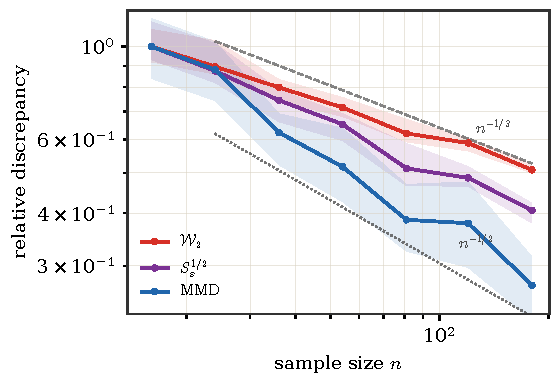
\includegraphics[width=.66\linewidth]{figures/sinkhorn-bias-variance-tradeoff/empirical-decay.pdf}
\caption{Empirical fluctuation in dimension three. For each sample size $n$, two independent empirical measures $\al_n$ and $\al'_n$ are drawn from the same standard Gaussian law in $\RR^3$. The curves show the median of $D(\al_n,\al'_n)$, normalized by its value at the smallest displayed $n$, with interquartile bands. Exact OT follows the slower dimension-dependent scale, while MMD and the fixed-$\epsilon$ Sinkhorn divergence behave closer to the parametric $n^{-1/2}$ guide. This is a statistical illustration, not a solver benchmark.}
\label{fig:sinkhorn-bias-variance-tradeoff}
\end{figure}

\begin{prop}[Empirical OT has dimension-dependent rates]\label{prop-empirical-ot-rate}
	Let $\alpha$ be a probability distribution with a density bounded above and below on $[0,1]^d$, and let $\hat\alpha_n=n^{-1}\sum_{i=1}^n\delta_{X_i}$ be its empirical measure. For $d>2p$, the typical scale of empirical OT is
	\[
		\EE\Wass_p(\hat\alpha_n,\alpha) \asymp n^{-1/d}.
	\]
	The exponent changes in low dimension, but the important message is that exact OT deteriorates with the ambient dimension.
\end{prop}

\begin{proof}
		We recall the standard multiscale argument, suppressing constants~\cite{dudley1969speed,fournier2015rate,weed2017sharp}. For the upper bound, partition $[0,1]^d$ into dyadic cubes. At scale $2^{-j}$, the empirical mass fluctuation over the cells is of order $n^{-1/2}2^{jd/2}$, while moving this excess mass inside cells costs $2^{-j}$. Summing the multiscale contributions up to the scale where the expected number of samples per cell is of order one gives $2^{-J}$ with $2^{Jd}\simeq n$, hence $n^{-1/d}$. For the lower bound, a packing argument shows that a positive fraction of cells at the critical scale are empty or overfull with non-negligible probability, forcing mass to travel at least a distance comparable to $n^{-1/d}$. The matching upper and lower bounds give the displayed rate.
\end{proof}

\begin{prop}[MMD has a parametric empirical rate]\label{prop-mmd-sample-rate}
	Let $k$ be a bounded positive definite kernel with RKHS $\Hh_k$, and define
	\[
		\MMD_k(\alpha,\beta)
		=
		\norm{\int k(x,\cdot)\d(\alpha-\beta)(x)}_{\Hh_k}.
	\]
	If $\hat\alpha_n$ is the empirical measure of $n$ i.i.d. samples from $\alpha$, then
	\[
		\EE\MMD_k(\hat\alpha_n,\alpha)^2
		=\frac{1}{n}\Big(\EE k(X,X)-\EE k(X,X')\Big),
	\]
	where $X,X'$ are independent with law $\alpha$. In particular, if $k(x,x)\leq \kappa^2$, then $\EE\MMD_k(\hat\alpha_n,\alpha)\leq \kappa/\sqrt n$.
\end{prop}

\begin{proof}
	Let $\Phi(x)=k(x,\cdot)$ be the feature map and $m_\alpha=\EE\Phi(X)$. Then
	\[
		\MMD_k(\hat\alpha_n,\alpha)
		=\norm{\frac1n\sum_{i=1}^n(\Phi(X_i)-m_\alpha)}_{\Hh_k}.
	\]
	Independence cancels the cross terms after taking the squared norm and expectation, giving
	\[
		\EE\MMD_k(\hat\alpha_n,\alpha)^2
		=\frac1n\EE\norm{\Phi(X)-m_\alpha}_{\Hh_k}^2
		=\frac{1}{n}\Big(\EE k(X,X)-\EE k(X,X')\Big).
	\]
	The last bound follows from Jensen's inequality and $k(x,x)\leq\kappa^2$.
\end{proof}

\begin{prop}[Sinkhorn divergences interpolate the rates]\label{prop-sinkhorn-sample-rate}
	Assume that $\alpha$ and $\beta$ are supported in a compact subset of $\RR^d$ and that the cost is smooth. For fixed $\epsilon>0$, debiased Sinkhorn divergences satisfy representative empirical bounds of the form
	\[
		\EE\abs{\bar\MK_c^\epsilon(\hat\alpha_n,\hat\beta_m)-\bar\MK_c^\epsilon(\alpha,\beta)}
		\leq
		C_{c,d}\,\epsilon^{-d/2}\left(\frac1{\sqrt n}+\frac1{\sqrt m}\right),
	\]
	up to constants and exponents depending on the precise smoothness class and support diameter. Thus regularization removes the $n^{-1/d}$ curse for fixed $\epsilon$, while the prefactor deteriorates as $\epsilon\to0$.
\end{prop}

\begin{proof}
	The proof follows the empirical-process argument of~\cite{genevay2018sample}. By the envelope theorem, the fluctuation of $\MK_c^\epsilon$ with respect to its first marginal is controlled by the class of entropic dual potentials. The soft $c$-transform smooths these potentials at spatial scale $\sqrt\epsilon$ for a quadratic-type cost. Covering a bounded $d$-dimensional domain at this scale gives an effective complexity of order $\epsilon^{-d/2}$. Standard Rademacher or Dudley entropy bounds then give an empirical-process fluctuation of order $\epsilon^{-d/2}/\sqrt n$ for each marginal. Applying the same estimate to the three terms defining the debiased divergence gives the stated bound.
\end{proof}

\begin{rem}[No free lunch when approximating exact OT]\label{rem-sinkhorn-no-free-lunch}
	The parametric rate in Proposition~\ref{prop-sinkhorn-sample-rate} holds for fixed $\epsilon$. If the goal is to approximate the unregularized OT value, one must also account for the regularization bias. In a typical bounded-cost finite-dimensional regime,
	\[
		\abs{\bar\MK_c^\epsilon(\alpha,\beta)-\MK_c(\alpha,\beta)}
		\leq C\epsilon,
		\qquad
		\EE\abs{\bar\MK_c^\epsilon(\hat\alpha_n,\hat\beta_n)-\bar\MK_c^\epsilon(\alpha,\beta)}
		\leq C_{c,d}\epsilon^{-d/2}n^{-1/2}.
	\]
	Balancing the two terms gives $\epsilon\simeq n^{-1/(d+2)}$ and total error of order $n^{-1/(d+2)}$. Equivalently, target accuracy $\eta$ requires choosing $\epsilon\simeq\eta$ and $n\simeq\eta^{-(d+2)}$ samples under this bound. Thus entropic smoothing improves the statistical behavior at fixed scale, but approximating exact OT still forces a bias-variance tradeoff whose exponent deteriorates with dimension.
\end{rem}
